% !TEX root = main.tex
\subsubsection*{사전 검증 후 로컬 Master Key 복구}
Committee 공개키·public share 자료는 사전에 검증해 보관한다.
타이머에는 받은 $k$개 share의 검증, Lagrange 보간, 복구한 키의 공개키 대조와 best-effort scalar 정리가 포함된다.
키 생성·DKG·통신·승인 대기는 제외한다.

전체 위원 수 $n=10$을 고정하고 $k$를 변화시켰다.
각 case는 warm-up 1,000회 후 공식 1,000회를 실행했으며, 공식 묶음의 전체 시간을 1,000으로 나눈 평균이다.
기존 5회 median과 섞지 않는다.
\begin{center}
    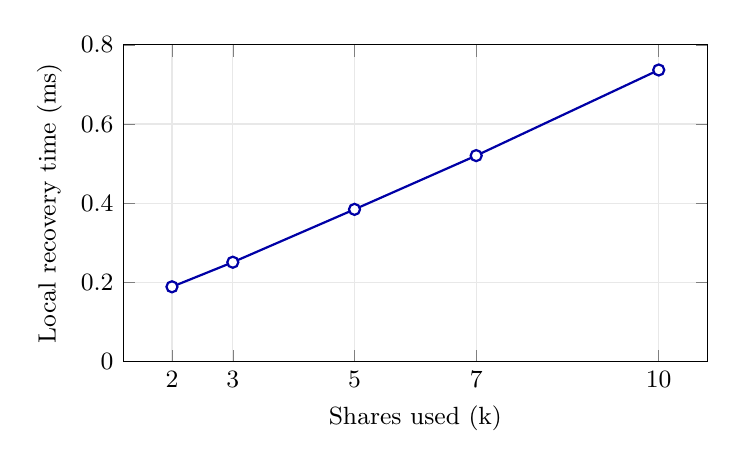
\begin{tikzpicture}\begin{axis}[width=7cm,height=5.6cm,grid=major,major grid style={gray!18},scaled ticks=false,tick label style={font=\small},label style={font=\small},width=9cm,xlabel={Shares used (k)},ylabel={Local recovery time (ms)},xtick={2,3,5,7,10},ymin=0,ymax=0.8]
            \addplot+[thick,mark options={fill=white},color=blue!65!black,mark=*] coordinates {(2,0.18843600000000002) (3,0.250553334) (5,0.38419966699999997) (7,0.520116083) (10,0.736622708)};
        \end{axis}\end{tikzpicture}\end{center}
{\small 그림 3. n=10 고정, k에 따른 로컬 복구 시간.}\par
\begin{center}\small\setlength{\tabcolsep}{6pt}
    \textbf{표 6. 사용 share 수에 따른 로컬 복구}\par\smallskip
    \begin{tabular}{@{}lr@{}}\toprule
        \textbf{k} & \textbf{시간 (ms)} \\ \midrule
        2          & 0.188            \\
        3          & 0.251            \\
        5          & 0.384            \\
        7          & 0.520            \\
        10         & 0.737            \\
        \bottomrule\end{tabular}\end{center}

이 구현은 타이머 안에서 전체 $n$명의 자료를 다시 순회하지 않는다.
따라서 이전의 $n$ 증가 그래프는 본문에서 제외했다. $n=10$이라는 실험 조건은 유지한다.
$k$가 늘면 검증할 share와 보간 연산량이 증가하지만, 이 값만으로 모든 시스템의 복잡도나 성능을 일반화하지 않는다.

이 측정은 Shamir share로 한 단계 감사 Master Key를 복구하는 비용이다.
논문 초안에서 별도 감사 데이터 키를 threshold encryption으로 감싸는 절차 전체의 비용이 아니다.
해당 두 키 구성의 성능으로 사용하려면 별도의 구현 대응과 측정이 필요하다.
    {\small 근거: prepared-recovery/result.json과 측정 경계 설명 [D4]. 각 case는 threshold에 맞는 유효한 share k개를 사용한다.}\par

